% =============================================================================
% P3D -- Privacidade 2: pôster (PT-BR)
% Formato: A3 retrato (297 x 420 mm), UMA página, Latin Modern.
% Figuras esperadas em out/: FigP1_PT.pdf, FigP3_PT.pdf (compiladas a partir de figuras/).
% O mapa de calor (Figura P2) é uma tabela colorida escrita neste arquivo.
% Conteúdo baseado em MD/P3D_Privacidade2_Poster_PT.md.
%
% Disposição: faixa de título; linha 1 = Figura P1 (esquerda) e Figura P2 (direita);
% linha 2 = Figura P3 em largura total; fechamento = uso e referências em largura total.
%
% UMA PÁGINA: todo o conteúdo fica dentro de uma única caixa (\parbox) envolvida por
% adjustbox com "max totalsize": se o conteúdo for mais alto que a página, ele é
% reduzido proporcionalmente até caber; se for menor, não é ampliado.
% Ajuste de tamanho: \corpo (texto), \figtitulo, \leitura, tamanho da tabela.
% Autores: editar o bloco \blocoautores.
% =============================================================================
\documentclass[12pt]{article}

\usepackage[T1]{fontenc}
\usepackage[utf8]{inputenc}
\usepackage{lmodern}
\usepackage[paperwidth=297mm,paperheight=420mm,margin=10mm]{geometry}
\usepackage[english,brazil]{babel}
\usepackage{graphicx}
\usepackage{xcolor}
\usepackage{array}
\usepackage{colortbl}
\usepackage[skins]{tcolorbox}
\usepackage{adjustbox}
\usepackage[expansion=false]{microtype}

\pagestyle{empty}
\setlength{\parindent}{0pt}
\setlength{\parskip}{0pt}
\raggedright

\definecolor{exLine}{RGB}{23,54,93}
\definecolor{exFill}{RGB}{220,233,247}
\definecolor{prFill}{RGB}{200,240,236}
\definecolor{prLine}{RGB}{8,127,140}
\definecolor{prText}{RGB}{6,79,87}
\definecolor{ctxText}{RGB}{38,52,67}

\newcommand{\corpo}{\fontsize{16}{21}\selectfont}
\newcommand{\figtitulo}[1]{{\centering\fontsize{16}{20}\selectfont\bfseries\color{exLine}#1\par}\vspace{2mm}}
\newcommand{\leitura}[1]{\vspace{2mm}{\fontsize{13}{17}\selectfont\color{ctxText}#1\par}}

% --- Autores, disciplina e código (editar aqui) ------------------------------
\newcommand{\blocoautores}{%
  \textbf{Autores:} Filipe Alves de Sousa, Emanuel Brandão de Galvão Correia, Ruben Isaac Dias da Silva e Carlos Eduardo da Silva Papa\\
  \textbf{Disciplina:} Gestão de Projetos de TI (GPTI) -- PPCA/CIC/UnB\\
  \textbf{Professores:} Dr. João Mello da Silva e Dr. Edison Ishikawa\\
  \textbf{Código:} 3p2 / 3R31}

\newtcolorbox{caixa}[1]{enhanced,colback=white,colframe=exLine,boxrule=0.5mm,arc=2mm,
  left=4mm,right=4mm,top=3mm,bottom=3mm,
  title={#1},fonttitle=\fontsize{18}{22}\selectfont\bfseries,coltitle=white,colbacktitle=exLine}

\begin{document}
\thispagestyle{empty}
\corpo

\noindent\begin{adjustbox}{max totalsize={\textwidth}{\textheight},center}
\parbox{\textwidth}{%
\raggedright

% ------------------------------- FAIXA ---------------------------------------
\begin{tcolorbox}[enhanced,colback=exLine,colframe=exLine,coltext=white,arc=2mm,
  left=6mm,right=6mm,top=4mm,bottom=4mm]
{\centering\fontsize{32}{37}\selectfont\bfseries PMBOK 8 em uma página\par}
\vspace{2.5mm}
\noindent\textcolor{white}{\rule{\linewidth}{0.5pt}}\par
\vspace{2.5mm}
\noindent\begin{minipage}[t]{0.48\linewidth}\raggedright
{\fontsize{18}{22}\selectfont\bfseries Princípios, processos e adaptação sob medida\par}
\vspace{1.5mm}
{\fontsize{14}{18}\selectfont Princípios orientam decisões; domínios e áreas de foco organizam o trabalho; \textit{tailoring} ajusta sua aplicação [4].\par}
\end{minipage}\hfill
\begin{minipage}[t]{0.48\linewidth}\raggedright
{\fontsize{13}{17}\selectfont\blocoautores\par}
\end{minipage}
\end{tcolorbox}

\vspace{4mm}

% ----------------------- LINHA 1: Figura P1 | Figura P2 -----------------------
\noindent
\begin{minipage}[t]{0.51\linewidth}
\raggedright
\figtitulo{Figura P1 --- Princípios e adaptação}
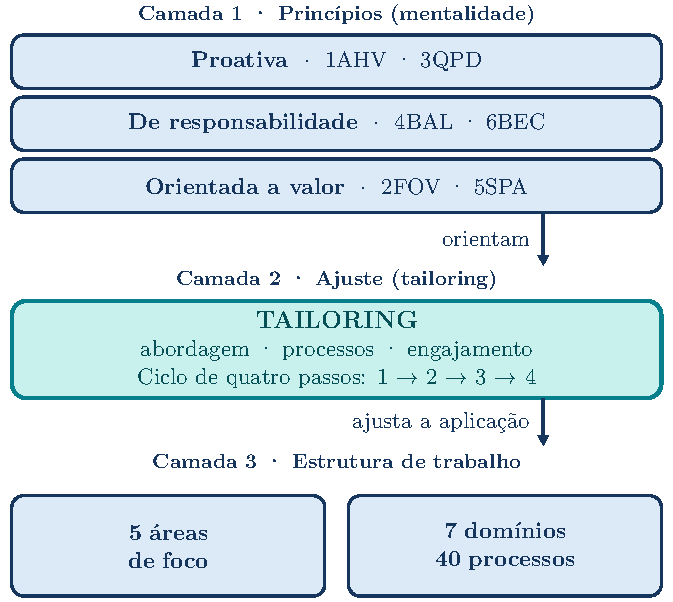
\includegraphics[width=\linewidth]{out/FigP1_PT.pdf}
\leitura{\textbf{Cinco operações sobre processos:} adicionar $\cdot$ modificar $\cdot$ remover $\cdot$ combinar $\cdot$ alinhar. \textbf{Três objetos da adaptação:} ciclo de vida e abordagem de desenvolvimento $\cdot$ processos $\cdot$ engajamento [4].}
\end{minipage}\hfill
\begin{minipage}[t]{0.44\linewidth}
\raggedright
\figtitulo{Figura P2 --- Mapa dos 40 processos}
{\fontsize{16}{21}\selectfont
\setlength{\tabcolsep}{4pt}
\renewcommand{\arraystretch}{1.45}
\noindent\begin{tabular*}{\linewidth}{@{\extracolsep{\fill}}lrrrrrr}
\hline
\textbf{Domínio} & \textbf{IN} & \textbf{PL} & \textbf{EX} & \textbf{MC} & \textbf{CL} & \textbf{Total}\\
\hline
Governança & \cellcolor{exLine!9}1 & \cellcolor{exLine!18}2 & \cellcolor{exLine!27}3 & \cellcolor{exLine!18}2 & \cellcolor{exLine!9}1 & 9\\
Escopo & 0 & \cellcolor{exLine!36}4 & 0 & \cellcolor{exLine!18}2 & 0 & 6\\
Cronograma & 0 & \cellcolor{exLine!18}2 & 0 & \cellcolor{exLine!9}1 & 0 & 3\\
Finanças & 0 & \cellcolor{exLine!27}3 & 0 & \cellcolor{exLine!9}1 & 0 & 4\\
Partes Interessadas & \cellcolor{exLine!9}1 & \cellcolor{exLine!18}2 & \cellcolor{exLine!18}2 & \cellcolor{exLine!18}2 & 0 & 7\\
Recursos & 0 & \cellcolor{exLine!18}2 & \cellcolor{exLine!18}2 & \cellcolor{exLine!9}1 & 0 & 5\\
Riscos & 0 & \cellcolor{exLine!36}4 & \cellcolor{exLine!9}1 & \cellcolor{exLine!9}1 & 0 & 6\\
\hline
\textbf{Total} & \textbf{2} & \textbf{19} & \textbf{8} & \textbf{10} & \textbf{1} & \textbf{40}\\
\hline
\end{tabular*}\par}
\leitura{\textbf{Legenda:} IN Iniciação $\cdot$ PL Planejamento $\cdot$ EX Execução $\cdot$ MC Monitoramento e Controle $\cdot$ CL Encerramento. Contagem de processos $\neq$ duração ou importância de uma área. \textit{Identify Stakeholders} está em Iniciação (Figura 2-32 do \textit{Guide}).}
\end{minipage}

\vspace{4mm}

% ----------------------- LINHA 2: Figura P3 (largura total) ------------------
\figtitulo{Figura P3 --- Quatro concentrações dos domínios}
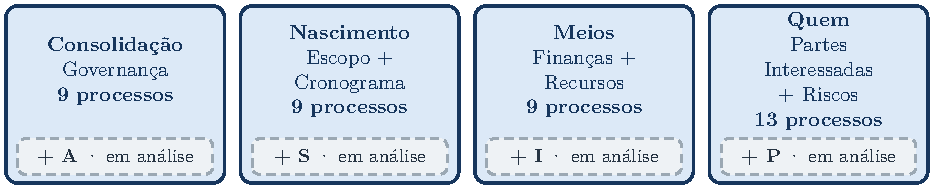
\includegraphics[width=\linewidth]{out/FigP3_PT.pdf}
\leitura{\textbf{Aviso de leitura:} as quatro concentrações e as etiquetas A, S, I e P são \textbf{agrupamento analítico adotado na disciplina GPTI/PPCA}; os sete domínios e seus 40 processos são do PMBOK 8 [4].}

\vspace{4mm}

% ----------------------- USO E FONTES EM LARGURA TOTAL -----------------------
\begin{caixa}{Como usar a síntese}
\corpo\raggedright
Escolha uma abordagem inicial, adapte-a à organização e ao projeto e melhore-a continuamente [4]. O mapa localiza os 40 processos, sem impor uma sequência única; a contagem por área não indica duração nem importância. O PMBOK 8 não descreve gêmeos digitais. Estudos sobre abordagens híbridas [3, 5] ajudam a contextualizar decisões de adaptação.
\end{caixa}

\vspace{4mm}

\begin{tcolorbox}[enhanced,colback=white,colframe=exLine,boxrule=0.5mm,arc=2mm,
  left=4mm,right=4mm,top=3mm,bottom=3mm]
{\fontsize{17}{21}\selectfont\bfseries\color{exLine}Referências principais}\hfill
{\fontsize{11}{14}\selectfont Numeração do relatório completo}\par\vspace{2mm}
{\fontsize{11}{15}\selectfont\raggedright
\begin{minipage}[t]{0.31\linewidth}\vspace{0pt}
[3] NOLL, J.; BEECHAM, S. How agile is hybrid agile? An analysis of the HELENA data. \textbf{PROFES 2019}, LNCS v. 11915, p. 341--349, 2019.
\end{minipage}\hfill
\begin{minipage}[t]{0.31\linewidth}\vspace{0pt}
[4] PMI. \textbf{The Standard for Project Management and A Guide to the PMBOK (PMBOK Guide)}. 8. ed., 2025. Documento de acesso restrito.
\end{minipage}\hfill
\begin{minipage}[t]{0.31\linewidth}\vspace{0pt}
[5] REED, A. et al. Usage of hybrid project management approaches and influences on approach selection. \textbf{Communications of the Association for Information Systems}, v. 54, 2024.
\end{minipage}}
\end{tcolorbox}

% AVISO-IA:INICIO
\vspace{2mm}
{\fontsize{10.5}{13}\selectfont\color{ctxText}\textbf{Uso de IA:} IA generativa (ChatGPT Astral 6 Sol e Sonnet 5.5, modo alto) apoiou a revisão de texto, a formatação, a criação de figuras e a formulação de tabelas. O grupo é responsável pelo conteúdo (COPE, 2023: \texttt{publicationethics.org/guidance/cope-position/authorship-and-ai-tools}).\par}
% AVISO-IA:FIM

}% fim do \parbox
\end{adjustbox}

\end{document}
